
\فصل{تعاریف و مفاهیم اولیه}

در این فصل به برخی مفاهیمی که در مسأله‌ی تحلیل بقا استفاده می‌شود می‌پردازیم. این مفاهیم در فصل‌های آتی استفاده می‌شود و به طور کلی در این زمینه تعریف‌شده و شناخته‌شده هستند. همچنین برخی از معیارهای بررسی کیفیت ومقایسه مدل‌های آنالیزگر بقا را شرح می‌دهیم . سپس در مورد جزئیاتی داده‌‌ها و نیز شیوه‌های کلی مدل‌های آنالیز بقا توضیحاتی ارائه خواهد شد.
%----------------------------- مقدمه ----------------------------------


\قسمت{توابع آنالیز بقا}
در تعاریف زیر از مقدار $t_i$ استفاده می‌شود. این مقدار برای بیمار شماره‌ی $i$، در صورتی که در اثر سرطان فوت کرده باشد، فاصله‌ی زمانی تشخیص تا فوت است و در صورتی که فوت نکرده باشد، فاصله‌ی زمانی تشخیص تا آخرین مراجعه‌‌ی بیمار می‌باشد.

یکی از اهداف مهم در آنالیز بقا، یافتن تابع بقاست \پاورقی{Survival Function}.
\شروع{تعریف}[تابع بقا \مرجع{r9}]
این تابع که آن را با
$S: \mathbb{R}^{+} \rightarrow \left[0, 1\right]$
نشان می‌دهیم، به این شکل تعریف می‌شود که اگر زمان فوت بیمار (پس از تشخیص بیماری) را با $T$ نشان دهیم، مقدار $S(t)$ برابر است با احتمال اینکه یک بیمار حداقل به اندازه $t$ پس از تشخیص زنده بماند. به بیان بهتر
$$S(t) = \mathbb{P}\left[T \geq t\right].$$
\پایان{تعریف}

این تابع می‌تواند برای یک بیمار و بر‌اساس ویژگی‌های او استخراج شود که در این صورت به فرم $S(t|x)$ خواهد بود که $x$ بردار ویژگی‌های بیمار است. همچنین می‌تواند به شکل جمعی و برای یک مجموعه از بیماران محاسبه شود. در این صورت تابع می‌تواند خطرناک بودن بیماری، نرخ مرگ و میر و متوسط عمر افراد فوتی را نمایش دهد. یکی از مدل‌‌هایی که برای تخمین تابع بقا به شکل جمعی استفاده می‌شود، \موکد{تخمین‌گر~\lr{Kaplan-Meier}} می‌باشد. این تخمین‌گر برای هر $t$، مقدار $S(t)$ را به شکل زیر حساب می‌کند:
$$S(t) = \prod_{i, t_i \leq t} (1-\frac{d_i}{n_i}).$$

که در رابطه‌ی بالا، $d_i$ برابر تعداد افرادی است که در لحظه‌ی $t_i$ مرده‌اند و $n_i$ تعداد افرادی است که تا پیش از لحظه $t_i$ زنده بوده‌اند.

\شروع{شکل}
[t]\centering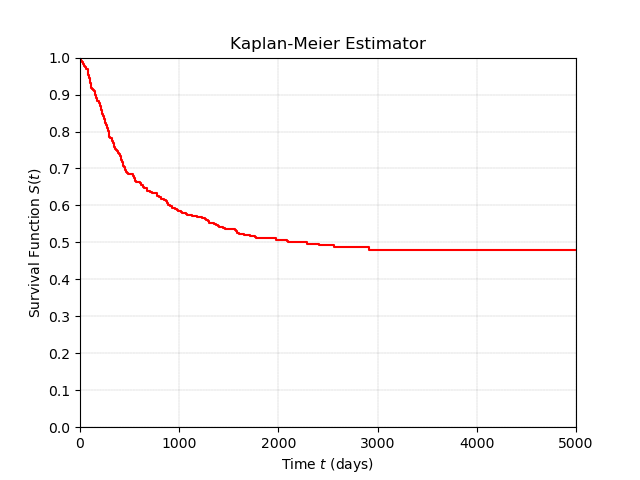
\includegraphics[width=250pt]{figs/kaplan-meier-estimator}

\شرح{تابع بقا؛ در اثر اجرای الگوریتم~\lr{Kaplan-Meier} روی کل داده‌ها}
\برچسب{شکل:تابع بقای جمعی}
\پایان{شکل}
	
با اجرای این الگوریتم روی کل داده‌ها، تابع بقا مطابق با شکل~\رجوع{شکل:تابع بقای جمعی} خواهد بود. همانطور که مشاهده می‌شود تقریباً نیمی از بیماران براساس داده‌های ما فوت نکرده‌اند، اما برای بیمارانی که فوت کرده‌اند، تابع بقا با شیب زیادی نزولی است که نشان می‌دهد بیماری کشنده بوده و در زمان کمی می‌تواند بیمار را از بین ببرد. 

\شروع{تعریف}[تابع خطر \پاورقی{Hazard Function} \مرجع{r9}]
تابع خطر که به صورت 
$h: \mathbb{R}^{+} \rightarrow \left[0, 1\right]$
تعریف می‌شود، قرار است میزان خطر در لحظه‌ی $t$ را معین کند. این تابع به صورت زیر محاسبه می‌شود:
$$h(t) = \mathbb{P}\left[t \leq T \leq t+\Delta t \ |\ T \geq t\right]
= \lim_{dt\rightarrow 0} \frac{\mathbb{P}\left[t\leq T\leq t+dt\right]}{\mathbb{P}\left[t \leq T\right]}
=
-\frac{S'(t) dt}{S(t)} = -\frac{d}{dt}\ln{S(t)}
$$
\پایان{تعریف}

تابع خطر همانطور که گفته شد، وقوع مرگ بیمار در لحظه $t$ را بررسی می‌کند. با این فرض که می‌دانیم بیمار تا لحظه‌ی $t$ زنده بوده است، می‌خواهیم ببینیم به چه احتمالی هم‌اکنون فوت می‌کند و در واقع خطر در لحظه‌ی $t$ برای بیمار چقدر است.


به شکل مشابه، تابع خطر تجمعی \پاورقی{Cumulative Hazard Function} نیز تعریف می‌شود.

\شروع{تعریف}[تابع خطر تجمعی \مرجع{r9}]
تابع تجمعی خطر که آن را به صورت 
$H: \mathbb{R}^{+} \rightarrow \left[0, 1\right]$
تعریف می‌کنیم، میزان خطر تا لحظه‌ی $t$ را حساب می‌کند. این تابع به شکل زیر محاسبه می‌شود:
$$H(t) = \int_{s=0}^t h(s) ds = -\ln{S(t)} + \ln{S(0))}
= -\ln{S(t)}$$
\پایان{تعریف}

تابع خطر تجمعی، می‌تواند میزان خطر تا لحظه‌ی $t$ را برای یک بیمار معین کند. در واقع اگر تابع بقای یک بیمار را داشته باشیم، تابع خطر جمعی، میزان خطر تجربه شده تا لحظه‌ی $t$ را نمایش می‌دهد. بعضی از مدل‌ها که در ادامه آن‌ها را معرفی خواهیم کرد، تابع $H(t | x)$ که در واقع تابع خطر تجمعی یک بیمار با بردار ویژگی‌های $x$ است را تخمین می‌زنند.

بر اساس تابع بالا، یک امتیاز ریسک \پاورقی{Risk Score} تعریف می‌شود که به کمک آن می‌توان بیماران مختلف یک مجموعه داده را با یکدیگر مقایسه کرد.

\شروع{تعریف}[امتیاز ریسک \مرجع{r9}]
امتیاز ریسک با داشتن تابع تجمعی خطر در $n$ نقطه‌ی مربوط به فوت یا آخرین مراجعه‌ی مجموعه‌ی بیماران محاسبه می‌شود (همان $t_i$ ها). این تابع که آن را برای بیمار با ویژگی‌های $x$ به شکل 
$R(x)$
نشان می‌دهیم. به شکل زیر محاسبه می‌شود:
$$R(x) = \sum_{i=1}^n H(t_i \ |\ x)$$
\پایان{تعریف}

اکنون برای مقایسه دو بیمار، می‌توانیم امتیاز ریسکشان را محاسبه کنیم و بیماری که امتیاز بالاتری کسب می‌کند، یعنی شدت بیماری برایش شدیدتر بوده و بیشتر در خطر است. برخی از مدل‌ها که در ادامه معرفی می‌شوند از این امتیاز ریسک برای ترتیب‌دهی به بیماران براساس شدت بیماری‌شان استفاده می‌کنند.

\قسمت{بررسی دقت مدل‌های آنالیز بقا}
در این قسمت می‌خواهیم به معرفی چندین معیار \پاورقی{Criteria} برای سنجش دقت مدل‌های آنالیز بقا بپرداریم. در فصل نتایج، از این معیارها جهت مقایسه و تحلیل مدل‌ها استفاده خواهد شد. محتوای این بخش براساس منبع \مرجع{r9} می‌باشد.

\شروع{تعریف}[معیار \lr{c-index} \پاورقی{Concordance index}]
این معیار، بر اساس پیش‌بینی $r_{i=1 ... n}$ مدل که میزان امتیاز ریسک بیماران را نشان می‌دهد، مقدار $C_{index}$ را بدین شکل محاسبه می‌کند:
$$C_{index}=\frac{
	\sum_{i, j}I(t_i>t_j, j\ \text{dead}, r_i<r_j)
	}{
	\sum_{i, j}I(t_i>t_j, j\ \textrm{dead})	
	}.$$
\پایان{تعریف}

در حقیقت معیار $C_{index}$، قرار است برای هر جفت $(i, j)$ که فرد $j$ فوت کرده باشد و فرد $i$ یا دیرتر از او مرده باشد، یا مطمئن باشیم که مدت طولانی‌تری عمر کرده است (براساس زمان آخرین مراجعه)؛ ببینیم که آیا مدل امتیاز ریسک درستی پیش‌بینی کرده است یا خیر. در حقیقت برای جفت $(i, j)$ که $j$ مرده باشد و $i$ عمر ببشتری کرده باشد، توقع داریم که مدلمان، امتیاز ریسک نفر $i$ را کمتر از امتیاز ریسک نفر $j$ پیش‌بینی کند. معیار $C_{index}$ در واقع نسبت تعداد جفت‌های $(i, j)$ ای است که مدل درست پیش‌بینی کرده به تعداد کل $(i, j)$ های معتبر. طبیعی است که مقدار $C_{index}$ عددی در بازه‌ی~$\left[0, 1\right]$ است و هر چه به $1$ نزدیک‌تر باشد، یعنی مدل بهتر توانسته است براساس داده‌ها، امتیاز ریسک بیماران را نسبت به هم پیش‌بینی کند. اگر یک مدل تصادفی داشته باشیم که امتیاز ریسک را به شکل تصادفی استخراج کند، مقدار $C_{index}$ برابر $0.5$ می‌شود.

\شروع{تعریف}[امتیاز Berier \پاورقی{Berier Score}]
معیار Berier در هر زمان $t$ طبق رابطه‌ی زیر محاسبه می‌شود:
$$BS(t) = \frac{1}{n}
\sum_{i=1}^n I(t_i \leq t, i\ \textrm{dead}) \frac{(0-S(t\ |\ x_i))^2}{G(t_i)}
+
I(t_i>t)\frac{(1 - S(t\ |\ x_i))^2}{G(t)}
.
$$
\پایان{تعریف}

این معیار در هر لحظه‌ی $t$ میزان خطای مدل را محاسبه می‌کند. برای این منظور، 
\شروع{فقرات}
\فقره
برای افرادی که تا لحظه‌ی $t$ فوت شده‌اند ($t_i \leq t$)،
مقدار 
$\frac{(0-S(t\ |\ x_i))^2}{G(t_i)}$
را به عنوان خطا در نظر می‌گیرد. علت این است که چون فرد $i$، پیش از لحظه‌ی $t$ مرده است، پس ما توقع داریم که تابع بقایی که برای او پیش‌بینی می‌کنیم به گونه‌ای باشد که پس از $t_i$، مقدار $S(t|x_i)$ بسیار کوچک و نزدیک $0$ باشد. به همین جهت مربع فاصله‌ی آن با $0$ را به عنوان خطا در نظر می‌گیریم.
\فقره
برای افرادی که تا لحظه‌ی $t$ فوت نشده‌اند ($t_i > t$)،
مقدار 
$\frac{(1 - S(t\ |\ x_i))^2}{G(t)}$
به عنوان خطا در نظر گرفته شده است. علت این است که چون فرد $i$ تا لحظه‌ی $t$ زنده بوده است، پس ما توقع داریم که تابع بقای‌ $S(t|x_i)$ تا آن لحظه مقداری نزدیک به $1$ داشته باشد. به همیت جهت مربع فاصله‌ی تابع با $1$ را به عنوان خطا در نظر می‌گیریم. نهایتاً میانگین خطاها برای همه‌ی افراد به عنوان $BS(t)$ گزارش می‌شود.
\پایان{فقرات}

در رابطه‌ی بالا، $G(t)$ برابر احتمال این است که داده‌ی سانسور شده (که در واقع زمان آخرین مراجعه‌ی بیمار است) که آن را با $C$ نشان می‌دهیم، بیشتر از $t$ باشد. به بیان بهتر
$G(t) = \mathbb{P}\left[C \geq t\right]$
است. همانطور که می‌بینید، تعریفی شبیه تابع بقا دارد و از
روش~\lr{Kaplan-Meier} برای تخمین آن استفاده می‌شود. همچنین با تجمیع مقدار امتیاز Berier روی همه‌ی زمان‌های ممکن، می‌توان امتیاز تجمعی Berier \پاورقی{Integrated Berier Score} را تعریف کرد.

\شروع{تعریف}[امتیاز تجمعی Berier ]
امتیاز تجمعی Berier که آن را با $IBS$ نشان می‌دهیم در بازه‌ی زمانی 
$\left[t_s, t_e\right]$
به صورت زیر محاسبه می‌شود:
$$\frac{1}{t_e-t_s} \int_{t_s}^{t_e} BS(t) dt.$$
\پایان{تعریف}
با کمک این امتیاز می‌توان معیار Berier را به شکل تجمعی روی  زمان‌های مختلف حساب کرد و از آن برای سنجش دقت مدل استفاده کرد. در حالت گسسته، انتگرال بالا تنها به ازای $n$ نقطه‌ی مربوط به $t_i$ ها محاسبه می‌شود و به کمک روش ذوزنقه‌ای \پاورقی{Trapezoidal} انتگرال محاسبه می‌شود. طبیعتاً هر چه امتیاز Berier کوچک‌تر باشد یعنی دقت مدل بهتر بوده است و بهتر توانسته که تابع بقا را براساس داده‌ها پیش‌بینی کند. اگر تابع بقا به شکل تصادفی ساخته شود، این معیار عددی در حدود $0.25$ خواهد داشت.

\شروع{تعریف}[امتیاز AUC \پاورقی{Cumulative Dynamic Area Under Curve}]
امتیاز AUC براساس خروجی امتیاز ریسک مدل برای بیماران که با 
$r_{i=1...n}$
نشان می‌دهیم، بدین شکل در لحظه‌ی $t$ محاسبه می‌شود:
$$AUC(t) =
\frac{\sum_{i, j} I(y_j>t) I(y_i\leq t, i\ \text{dead}) w_i I(r_i > r_j)}
{\sum_{i, j}I(y_j>t) I(y_i\leq t, i\ \textrm{dead}) w_i}.$$
که در رابطه‌ی بالا
 $w_i=\frac{1}{G(t_i)}$
است.
\پایان{تعریف}

این معیار در لحظه‌ی $t$، بیمارانی که تا لحظه‌ی $t$ فوت شده‌اند و بیمارانی که مطمئنیم حداقل تا لحظه‌ی $t$ زنده بوده‌اند را جفت می‌کند و امتیاز بالا می‌رود اگر مدل ما امتیاز ریسک را برای این جفت‌ها به درستی محاسبه کرده باشد. طبیعتاً این امتیاز هر چه به $1$ نزدیک‌تر باشد، یعنی دقت مدل بیشتر است. مشابه بالا می‌توانیم امتیاز AUC تجمیعی را هم در بازه‌ی~$\left[t_s, t_e\right]$
بدین شکل محاسبه کرد:
$$AUC = \frac{1}{t_e-t_s} \int_{t=t_s}^{t=t_e} AUC(t) dt.$$


\قسمت{مقدمه‌ای بر روش‌های آنالیز بقا}
روش‌های آنالیز بقا امروزه عمدتاً با یادگیری ماشین عجین شده‌اند. اما روش‌های کلاسیک هم همچنان استفاده می‌شوند. یکی از این روش‌های معروف شیوه‌ی \lr{Cox-PH} است. این روش براساس داده‌ها تابع خطر را برای یک بیمار در هر لحظه‌ی $t$ محاسبه می‌کند.

اما روش‌های یادگیری ماشین که به خاطر توانایی‌شان در استخراج دانش از داده‌ها در ابعاد بالا امروزه بیش از پیش مورد توجه قرار گرفته‌اند، در اشکال و انواع گوناگونی در آنالیز بقا هم به کار گرفته می‌شوند.
شیوه‌های مبتنی بر یادگیری ماشین در آنالیز بقا، به طور کلی در $4$ دسته قرار می‌گیرند \مرجع{r9}. 

مدل‌های دسته‌ی نخست، مبتنی بر جنگل‌های تصادفی \پاورقی{Random Forests} می‌باشند که با تجمیع تعداد زیادی مدل ساده‌تر به نام درخت تصمیم \پاورقی{Decision Tree}، از پیش‌بینی همگی آن مدل‌ها استفاده می‌کنند و ترکیبی از خروجی مدل‌ها را به عنوان نتیجه نهایی اعلام می‌کنند. این فرایند را تجمیع خود راه‌انداز\پاورقی{Bagging} می‌گویند. نکته‌ی قوت این مدل‌ها در سادگی پیاده‌سازی و نیز تفسیرپذیری‌شان است \مرجع{r11}. 

دسته دوم از مدل‌ها، مبتنی بر ماشین‌های تقویت گرادیان\پاورقی{Gradient Boosting} است. ایده‌ی تقویت در یادگیری ماشین بدین صورت است که یک مدل قوی می‌تواند در اثر تجمیع تعدادی مدل ضعیف \پاورقی{Weak Learner} ایجاد شود. تفاوت این دسته از مدل‌ها، با مدل‌های دسته‌ی نخست این است که در جنگل‌های تصادفی، هر یک از درخت‌های تصمیم به شکلی مستقل از روی داده چیزی می‌آموزند اما در این دسته از مدل‌ها، مدل‌های ضعیف‌‌تر به شکل متوالی آموزش داده می‌شوند و هر کدام براساس مدل‌های پیشین خود آموزش می‌بینند.  نهایتاً ترکیبی خطی از خروجی این مدل‌های ضعیف، خروجی نهایی را تولید می‌کند \مرجع{r9, r11}. 

دسته‌ی سوم از مدل‌ها، مبتنی بر ماشین بردار پشتیبانی \پاورقی{Support Vector Machine} می‌باشند. این مدل‌ها سعی می‌کنند که به نحوی بقای بیماران را به شکلی خطی تخمین بزنند. برخی از مدل‌های این دسته سعی می‌کنند رتبه‌بندی مناسبی از بیماران ارائه دهند.

نهایتاً در دسته‌ی آخر، شبکه‌های عصبی را داریم که قابلیت تخمین توابع بسیار پیچیده را دارند. تعیین تابع هزینه \پاورقی{Loss Function} در این مدل‌ها بسیر حائز اهمیت است. برخی از این مدل‌ها، توابع هدف را به شکل گسسته و برخی به شکل پیوسته پیش‌بینی می‌کنند. مدل‌های گوناگونی امروزه برای آنالیز بقا پیش‌نهاد شده‌اند \مرجع{r7, r6, r12, r13, r14, r15} که ما برخی از آن‌ها را بررسی خواهیم کرد.

در فصل مدل‌ها، ما به بیان دقیق‌تر مدل‌هایی که روی داده‌هایمان استفاده کردیم خواهیم پرداخت و در فصل نتایج عملکرد آن‌ها را بررسی می‌کنیم.

\حذف{
\شروع{تعریف}
یک الگوریتم تقریبی برای مسئله‌ی $P$ 
دارای \موکد{ضریب تقریب افزایشی}\پاورقی{additive approximation factor} $c$ است 
اگر برای هر نمونه‌ی $I$ از~$P$:

\[
	|ALG(I) - OPT(I)| \leq c. 
\]
\پایان{تعریف}
} %پایان حذف

\قسمت{داده‌ها}
همانطور که اشاره‌شد، ما داده‌های $526$ بیمار مبتلا به سرطان دهان را جمع‌‌آوری کردیم.
در داده‌هایمان، ما تعدادی فیلد تهی\پاورقی{Null} داشتیم که برای پر کردن داده‌های خالی از روش $k$~نزدیک‌ترین~همسایه
\پاورقی{$k$-Nearest Neighbors (KNN)}
با $k=11$ بهره گرفته شد.
برای هر بیمار $22$ ویژگی داریم که توضیحات آنها به شرح زیر است.
\شروع{فقرات}
\فقره
داده‌های دودویی
\شروع{فقرات}
\فقره کاهش وزن رخ داده است؟ (\lr{Weight loss})
\فقره آیا غدد لنفاوی درگیر شده‌اند؟ (\lr{Lymph node involvement})
\فقره آیا پرتو‌درمانی انجام شده است؟ (\lr{Radiotherapy})
\فقره آیا جراحی انجام شده است؟ (\lr{Surgery})
\فقره آیا شیمی‌درمانی انجام شده است؟ (\lr{Chemotherapy})
\فقره آیا برداشت توده انجام شده است؟ (\lr{Resection})
\فقره آیا برداشت توده با برش گردن انجام شده است؟ (\lr{Resection with neck dissection})
\فقره وضعیت حاشیه (\lr{Margin status})
\فقره آیا بیمار مراجعه‌ی مجدد داشته؟ (\lr{Regular follow up})
\فقره آیا عود رخ داده؟ (\lr{Recurrence})
\فقره آیا عود شیمی‌درمانی شده؟ (\lr{Chemotherapy after recurrence})
\فقره آیا عود رادیوتراپی شده؟ (\lr{Radiotherapy after recurrence})
\فقره آیا عود جراحی شده؟ (\lr{Surgery after recurrence})
\فقره آیا متاستاز رخ داده است؟ (\lr{Metastasis})
\فقره آیا بدخیمی ثانویه رخ داده است؟ (\lr{Second primary malignancy})
\فقره \مهم{بیمار فوت شده است؟} (\lr{Death})
\پایان{فقرات}
\فقره
داده‌های دسته‌ای \پاورقی{Categorical}
\شروع{فقرات}
\فقره محل اولیه‌ی درگیری (\lr{Site})
\فقره سطح هیستولوژیکال (\lr{Histologic grade})
\فقره زمان عود (\lr{Recurrence time})
\پایان{فقرات}
\فقره داده‌های عددی \پاورقی{Numerical}
\شروع{فقرات}
\فقره سایز تومور (\lr{Tumor size})
\فقره تعداد غدد لنفاوی درگیر (\lr{Number of involved lymph nodes})
\فقره سن (Age)
\فقره \مهم{فاصله‌ی زمانی بین تشخیص تا آخرین مراجعه یا فوت} 
\پایان{فقرات}
\پایان{فقرات}

\قسمت{جمع‌بندی}
در این فصل، نخست به بیان توابعی که در آنالیز بقا به کار می‌روند، پرداختیم و تابع بقا، تابع خطر، تابع خطر تجمعی و امتیاز ریسک را معرفی کردیم. سپس معیارهایی را که در سنجش عملکرد مدل‌ها در آنالیز بقا استفاده می‌شوند شرح دادیم و توضیحاتی در خصوص معیار c-index ، امتیاز Berier و امتیاز AUC ارائه شد. در ادامه دسته‌بندی کلی‌ای بر روش‌های موجود در آنالیز بقا بیان شد و نهایتاً داده‌هایمان در انتهای فصل توصیف شدند.





